\section{Model celowania w grze Phoenix Point (Bartosz Strzelecki)}

W Phoenix Point modelowanie dokładności to wieloaspektowy system, który w zawiły sposób definiuje wynik interakcji bojowych. 
Gra wykorzystuje dynamiczny system celowania, który uwzględnia różne elementy, takie jak postawa żołnierza, biegłość w posługiwaniu się bronią, zasięg, 
osłona i warunki środowiskowe, aby określić celność strzału. Każdy z tych elementów odgrywa znaczącą rolę w ogólnym obliczeniu trafienia w cel.

W przeciwieństwie do podobnej gry XCOM, gdzie celność jest zamodelowana za pomocą prostej szansy na trafienie, w grze Phoenix Point
trajektoria każdego pocisku obliczana jest osobno. Podczas celowania widoczne są dwa okręgi: wewnętrzny, który reprezentuje miejsce,
w którym znajdzie się 50\% pocisków oraz zewnętrzny, który reprezentuje maksymalny rozrzut broni. W tym przypadku im celniejsza broń, tym
okręgi będą mniejsze.
\begin{figure}[h]
\centering
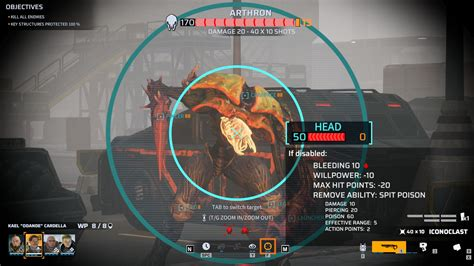
\includegraphics[width=0.6\textwidth]{images/point}
\caption{System celowania występujący w grze Phoenix Point.}
\label{fig:acc}
\end{figure}
